\documentclass[sigconf]{acmart}


\usepackage{xcolor}

\usepackage{float}
\usepackage{siunitx}


\newif\iffinal

% \finaltrue

\iffinal
  \newcommand{\tyler}[1]{}
  \newcommand{\ian}[1]{}
  \newcommand{\kyle}[1]{}
  \newcommand{\ryan}[1]{}
  \newcommand{\logan}[1]{}
\else
  \newcommand{\tyler}[1]{{\textcolor{cyan}{ tyler: #1 }}}
  \newcommand{\ian}[1]{{\textcolor{red}{ Ian: #1 }}}
  \newcommand{\kyle}[1]{{\textcolor{purple}{ Kyle: #1 }}}
  \newcommand{\ryan}[1]{{\textcolor{magenta}{ Ryan: #1 }}}
  \newcommand{\logan}[1]{{\textcolor{olive}{ Logan: #1 }}}
\fi


%%
%% \BibTeX command to typeset BibTeX logo in the docs
\AtBeginDocument{%
  \providecommand\BibTeX{{%
    \normalfont B\kern-0.5em{\scshape i\kern-0.25em b}\kern-0.8em\TeX}}}


\newcommand{\name}{Xtract}
\newcommand{\funcx}{$f$\kern-0.18em\emph{unc}\kern-0.05em X}

\acmConference{Fifth International Workshop on Serverless Computing (WoSC)}{2019}{Davis, CA}

\begin{document}


\title{Serverless Workflows for Indexing Large Scientific Data}


\author{Tyler J. Skluzacek} 
\affiliation{University of Chicago}
\email{skluzacek@uchicago.edu}

\author{Ryan Chard}
\affiliation{Argonne National Laboratory}
\email{rchard@anl.gov}

\author{Ryan Wong}
\affiliation{University of Chicago}
\email{rewong03@uchicago.edu}

\author{Zhuozhao Li} 
\affiliation{University of Chicago}
\email{zhuozhao@uchicago.edu}

\author{Yadu N. Babuji}
\affiliation{University of Chicago}
\email{yadunand@uchicago.edu}

\author{Logan Ward}
\affiliation{Argonne National Laboratory}
\email{lward@anl.gov}

\author{Ben Blaiszik} 
\affiliation{Argonne National Laboratory}
\email{bblaiszik@anl.gov}

\author{Kyle Chard}
\affiliation{University of Chicago}
\email{chard@uchicago.edu}

\author{Ian Foster}
\affiliation{Argonne \& University of Chicago}
\email{foster@anl.gov}



\renewcommand{\shortauthors}{Skluzacek et al.}

\begin{abstract}

%Advances in scientific instruments and the increased proliferation of IoT devices and sensors 
%lead to the ever-growing variety, velocity, and volume of scientific data. 
%Increased data combined with the adoption of data-driven methodologies has 
%resulted in a desire to capture and store vast amounts of data for long periods of time.
%To obtain the greatest utility from these data they must be adequately described
%and organized such that researchers can find, understand, and explore them.

%The data stored in scientific data repositories, file systems, and data stores 
%are only as useful as the metadata available to describe those data. 
%Data lakes are an increasingly common approach for storing and managing collections of scientific data. 
%Unlike structured approaches, data lakes integrate data from various sources and 
%use associated metadata to make them both discoverable and usable. 
%However, due to growing data volumes, distributed collaborations, and a desire to store data for long periods of
%time, such ``data lakes'' quickly become disorganized, lacking the metadata necessary to be useful to researchers. 
%Given the quantity of stored data, it is no longer possible to manually describe, curate, and organize data. 
%Instead, automated methods are needed to extract and associate suitable metadata.
%In addition, the size of many scientific datasets can be prohibitively large
%to transfer and require metadata extraction to be performed at the edge.
%\kyle{I havent read the paper yet, but I imagine we might want to make the argument
%that we want to do extraction at the edge as its not possible to move the data.} 

The use and reuse of scientific data is ultimately dependent on 
the ability to understand what those data represent, how they were 
captured, and how they can be used.  In many ways, 
data are only as useful as the metadata available to describe them.
Unfortunately, due to growing data volumes, large and distributed collaborations, 
and a desire to store data for long periods of time, scientific ``data lakes'' 
quickly become disorganized and lack the metadata necessary to be useful to researchers.
%It is both time-consuming and expensive to manually describe, curate, and organize data. 
%The increasing volume, velocity, and variety of scientific data makes it cost-prohibitive for 
%researchers to manually describe and curate data. 
%Instead automated methods for deriving and associating metadata with data.
New automated approaches are needed to derive metadata from scientific files
and to use this metadata for organization and discovery.
Here we describe one such system, \name{}, a service capable of processing vast
collections of scientific files and automatically extracting metadata from diverse
file types. \name{} relies on function as a service models to enable
scalable metadata extraction by orchestrating the execution of many, short-running
metadata extraction functions. To reduce data transfer costs, \name{} can 
be configured to deploy extractors centrally or near to the data (i.e., at the edge).
%\name{} can be applied to remote datasets and will dynamically crawl, stage, 
%and process data, resulting in a curated and searchable index of metadata for a dataset.
%\name{} builds upon a function-as-a-service platform, enabling metadata extraction
%tasks to be applied to data at the edge.
We present a prototype implementation of \name{} and demonstrate that it can 
derive metadata from a 7 TB scientific data repository. 
% We show it can derive a search index of data in less than one day.
%\ryan{With this edge focus should we rename to Xtract rather than \name{}?}

\end{abstract}


%%
%% The code below is generated by the tool at http://dl.acm.org/ccs.cfm.
%% Please copy and paste the code instead of the example below.
%%
\begin{CCSXML}
<ccs2012>
<concept>
<concept_id>10002951.10003227.10010926</concept_id>
<concept_desc>Information systems~Computing platforms</concept_desc>
<concept_significance>500</concept_significance>
</concept>
<concept>
<concept_id>10002951.10003317.10003365.10003366</concept_id>
<concept_desc>Information systems~Search engine indexing</concept_desc>
<concept_significance>300</concept_significance>
</concept>
<concept>
<concept_id>10002951.10003317.10003318.10003319</concept_id>
<concept_desc>Information systems~Document structure</concept_desc>
<concept_significance>100</concept_significance>
</concept>
<concept>
<concept_id>10010405.10010497.10010500.10010503</concept_id>
<concept_desc>Applied computing~Document metadata</concept_desc>
<concept_significance>500</concept_significance>
</concept>
</ccs2012>
\end{CCSXML}

\ccsdesc[500]{Information systems~Computing platforms}
\ccsdesc[500]{Applied computing~Document metadata}
\ccsdesc[300]{Information systems~Search engine indexing}
\ccsdesc[100]{Information systems~Document structure}

\keywords{data lakes, serverless, metadata extraction, file systems, materials science}

\maketitle

\section{Introduction}

Advances in scientific instruments, computational capabilities, and the proliferation of IoT devices
have increased the volume, velocity, and variety of research data. 
As a result, researchers are increasingly adopting data-driven research practices, 
in which data are collected, stored for long periods of time, shared, 
and reused.
Unfortunately, these factors create new research data management challenges, 
not least of which is the need for data to be adequately described
for it to be generally useful. Without descriptive metadata, data
may become unidentifiable, siloed, and in general, 
not useful to either the researchers who own the data or the broader scientific community. 
Unfortunately, organizing and annotating data is a time-consuming process
and the gulf between data generation rates
and the finite management capabilities of researchers
continues to grow. % resulting in an explosion of mismanaged data. 
To increase the value and usefulness of scientific data, 
new methods are required to automate the extraction and association 
of rich metadata that describe not only the data themselves, but
also their structure and format, provenance, and administrative information.

%Scientific discovery is increasingly collaborative, and distributed, in nature. While such teamwork has proven to 
%increase scientific efficiency and research novelty~\cite{presser1980collaboration}, it also results in large, schemaless
%collections of research artifacts (e.g., data, academic papers, and analysis scripts) called `data lakes'
%~\cite{miloslavskaya2016big}. 
Data lakes have become a popular paradigm for managing large and 
heterogeneous data from various sources. 
A data lake contains a collection of data in different formats, 
accompanied by metadata describing those data. % making the entire data collection usable and useful. 
Unfortunately, the data deluge and the desire to store all data
for eternity can quickly turn a data lake into a ``data 
swamp''~\cite{skluzacek2018skluma}---a term used to describe the situation in which the data 
stored in the data lake lack the metadata necessary to be 
discoverable, understandable, and usable. Without automated and scalable 
approaches to derive metadata from scientific data, the utility of 
these data are reduced. This problem is 
especially prevalent in science as 
datasets can be enormous (many petabytes),
are created and shared by dynamic collaborations, 
are often collected under tight time constraints where data management processes become afterthoughts, 
and for which preservation is important for purposes of reproducibility and reuse. 

Extracting metadata from scientific data is a complex task. 
Scientific repositories may exceed millions of files and petabytes of data;
data are created at different rates, by different people; 
and there are an enormous number of data formats and conventions. 
While metadata can be rapidly extracted from some data types, others, such as
images and large hierarchical file formats can require the use of multiple extraction methods.  
As a result, the metadata extraction process must be scalable to process large numbers
of files, flexible to support different extraction methods, and extensible
to be applied to various scientific data types and formats.

Serverless computing, and in particular function as a service (FaaS),
provides an ideal model for managing the execution of
many short-running extractors on an arbitrarily large number of files. 
Serverless computing abstracts computing resources from the user, enabling
the deployment of applications without consideration for the physical and virtual infrastructure on which 
they are hosted. %All infrastructure is instead managed automatically by the serverless computing provider.  
%The most well-known serverless model, Function-as-a-Service (FaaS), 
FaaS allows users to register programming functions with predefined input signatures. 
Registered functions can subsequently be invoked many times
without the need to provision or scale any infrastructure.
%Instead, operating and scaling the
%infrastructure performing tasks. Serverless is especially applicable for creating 
%customizable metadata extraction 
%workflows that can be applied to data regardless of their location.
%both at the edge (i.e., at the data) and as a service on a dedicated computing cluster.

In this paper we propose the use of FaaS for mapping the metadata extraction problem to a 
collection of granular metadata extractor functions. 
 %that are executable on
%serverless computing platforms. 
We describe how such a model can support the flexibility, scalability, and extensibility required
for scientific metadata extraction. 
Rather than rely on commercial FaaS systems, we use a distributed FaaS model 
that overcomes the limitation of moving large amounts of data to the cloud. 
Instead, we are able to push
%We also explore one of the biggest limitations of commercial FaaS systems, that is, the need
%to upload data to the cloud. Instead, we explore a FaaS-at-the-edge model in which 
metadata extractors to the edge systems on which the scientific data reside. 

Our prototype system, \name{}, provides high-throughput and on-demand metadata 
extraction that enables the automated creation of rich, searchable data lakes from previously unsearchable data swamps. 
\name{} implements dynamic metadata extraction workflows comprised of serverless functions that may be 
executed in the cloud or at the edge. \name{} runs as a centralized management
service that orchestrates the crawling, transfer (when necessary), and execution of 
metadata extraction functions. % and outputs a rich metadata. 
\name{} uses the \funcx{} serverless supercomputing platform~\cite{chard2019serverless}
to execute functions across diverse and distributed computing infrastructure.
We evaluate \name{}'s performance by extracting metadata from materials
science data stored in the 7~TB Materials Data Facility (MDF)~\cite{blaiszik2016materials, blaiszik2019mdf}. 

The remainder of this paper is organized as follows. 
\S\ref{sec:swamp} outlines example scientific data lakes. 
\S\ref{sec:xtracthub} describes \name{}'s serverless architecture and presents the set of available extractors.
\S\ref{sec:eval} provides initial results of system performance on hundreds of thousands of scientific files.
Finally, \S\ref{sec:related} and \S\ref{sec:conclusion} present related work and concluding remarks, respectively. 


\section{Scientific Data Lakes}
\label{sec:swamp}

Data lakes are schemaless collections of heterogeneous files obtained from different sources. 
Unlike traditional data warehouses, data lakes do not require upfront schema integration and instead allow 
users to store data without requiring complex and expensive Extract-Transfer-Load (ETL) pipelines. 
This low barrier to data archival encourages the storage of more bytes and types of data. 
However, the lack of a well-defined schema shifts responsibility from upfront integration
to descriptive metadata to allow users to search, understand, and use the data. 
To motivate our work we briefly describe three scientific data lakes below. 

%Expecting scientists to manually curate metadata for 
%this catalog can prove futile~\cite{jagadish2014big}, resulting in data becoming lost or unusable in the `data swamp'. 
%Dredging a data swamp typically involves sifting through giga-, tera-, or petabytes of data and using 
%automated workflows to extract, derive, and validate metadata about each file. The 
%remainder of this section outlines three examples of scientific data lakes found in the wild.   

%\kyle{This seems like a slight leap - collaborations == data lakes. I think
%the intro motivates the adoption of data lakes as an idea fairly well so perhaps don't need to get into it
%again. Maybe move the collaboration refs into the intro?}
%For instance, data might be collected from thousands of 
%edge devices, intermediately processed by a computing cluster, and the raw data delivered to a number of geo-distributed 
%collaborators. As an increasing number of devices and personnel edit and augment research artifacts (e.g., files), 
%finding and using data from the data lake becomes increasingly dependent on the metadata and some index or catalog
%of said artifacts. 
%However, 
The \emph{Carbon Dioxide Information Analysis Center (CDIAC)}
%There are many well-defined cases of institutions using metadata extraction workflows to take existing data swamps and 
%turn them into rich research data lakes. 
%As recently as 2017, the Carbon Dioxide Information Analysis Center (CDIAC) 
collected a dataset of emissions data from the 1800s through 2017.
The dataset contains more than \num{500000} files (330+ GB) 
with over \num{10000} unique file extensions. 
The archive contains little descriptive metadata 
and includes a number of irrelevant files, such as 
as debug-cycle error logs and Windows desktop shortcuts.
The data are currently being moved to the  
Environmental System Science Data Infrastructure for a Virtual Ecosystem (ESS-DIVE) archive~\cite{essdive}.
In prior work we extracted metadata from files in this repository
and created a data lake for users~\cite{skluzacek2016klimatic, skluzacek2018skluma}.

\emph{DataONE~\cite{michener2011dataone}} provides access to a distributed network
of biological and environmental sciences data repositories. 
DataONE manages a central index across these distributed repositories, enabling users
to discover datasets based on metadata queries. 
Member data repositories provide dataset- and file-level metadata to DataONE.
As of May 2019, DataONE contains over 1.2 million files and \num{809000} unique metadata entries. 

The \emph{Materials Data Facility (MDF)}~\cite{blaiszik2016materials, blaiszik2019mdf}
is a centralized hub for publishing, sharing, and discovering materials science data. 
The MDF stores many terabytes of data from many different research groups, covering many disciplines of 
materials science, and with a diverse range of file types.
The downside of the expansive range of materials data held by the MDF 
is that it can be difficult for users to find data relevant to their science.
The MDF reduces the ``data discovery" challenge by hosting a search index that provides access to metadata from the 
files (e.g., which material was simulated in a certain calculation).
The data published by the MDF is primarily stored on storage at the National Center for Supercomputing Applications
(NCSA) and is accessible via Globus. 


\section{Xtract}
\label{sec:xtracthub}%absolutely

\name{} is a metadata extraction system that provides on-demand extraction
from  heterogeneous scientific file formats. 
%tools to scientists who wish to make their data readily accessible, findable, and usable by the wider research community. 
\name{} can operate in one of two modes: centralized or edge metadata extraction. 
In the centralized mode, \name{} processes files stored on a Globus endpoint by first staging
them to a centralized location and then executing metadata extraction pipelines on those files. 
In the edge mode, \name{} can execute metadata extraction pipelines on edge computers near
the data by deploying a collection of metadata extraction functions to distributed FaaS endpoints. 
%communicates with endpoint agents to perform metadata extraction tasks on diverse computing machinery, 
%from laptops to the cloud to HPC centers. \name{} can be applied to any accessible Globus endpoint.
%When invoked, \name{} initializes by crawling the Globus endpoint and creating a list of files to be processed. Based on 
%a user's preference, \name{} can proceed in one of two ways: either staging remote files to the \name{} service, or transmitting
%metadata extraction functions to the data. 
%extract metadata at-the-edge or first transfer the files to a dedicated 
%computing resource. 

In order to extract metadata, \name{} applies various extractors---functions that take a file as input 
and generate a JSON document of metadata for that file. 
%In the centralized mode, data is staged to the \name{} service by initiating Globus transfer requests 
%to move data to a temporary data store for processing. 
%It later deletes the file after it has been processed.
%In edge mode, extraction is achieved by deploying a FaaS agent to perform extraction functions on the remote resource. 
%Once deployed, \name{} will send metadata extraction functions to the data for execution. 
In either centralized or edge mode, \name{} assembles a pipeline of extraction functions based on
file contents and metadata extracted from other extractors. 
\name{} begins the process of extracting metadata by first applying 
a file type extractor which informs selection of subsequent extractors. 
Subsequent extractors are selected based on their expected metadata yield. 
This allows \name{} to apply the appropriate extractors to a specific file. 

\name{} creates a metadata document for each file it processes. When an extractor is applied
to a file, \name{} appends the extractor's output metadata to the file's metadata document.
Once all of the data are processed the metadata document is ingested into a Globus 
Search index~\cite{ananthakrishnan2018globus}. 


\subsection{Extractors}

\name{} includes extractors for many file types commonly used in science. 
Each extractor is implemented as either a Python function or Bash script. 
%\ryan{Our final future work sentence says we will do this later. Do we remove here or there?}
The remainder of this section outlines \name{}'s library of extractors and
the data types they have been designed to process. 

\textbf{The universal extractor}
extracts generic file information such as file extension,
path, and size. It also computes an MD5 hash (for duplicate detection). 
The universal extractor is typically the first executor applied to a 
file. 

%\kyle{I'm a bit confused by this extractor. I think it is doing 2 things? 
%1) taking a sample of bytes and inferring a type (e.g., text or image)? 
%2) Testing all extractors and building a model of type (maybe text or image) to what extractors provide metadata?}
%\kyle{What features are used to build this model? is it just the 512 bytes -> type -> extractor?}
%\kyle{Why is it not pretrained? This seems like an annoyance that 
%we'd have to run on a bunch of files before even being able to run the inference?}

%\tyler{how's this? (below)}
\textbf{The file type extractor} applies a machine learning model to 
infer the type of a file. This information is crucial for determining  which
downstream extractors could yield metadata from that file. 
Users can opt to use a pre-trained model, or to automatically train one on
their data. In the latter case, training commences by selecting $n$\% of the files in the 
repository at random and running those files through all other \name{} extractors. 
We record whether or not the extractor produces metadata and build a 
\emph{file} $\rightarrow$ \emph{extractor} label mapping based on those that yield metadata.
It then trains a random forests model using these labels and the first 512 bytes of the file as features.
The primary goal of this extractor is to save time---the amount of time to incorrectly apply metadata extractors to a 
file can take seconds, whereas predicting which extractors will likely produce metadata
via the byte footprint of a file is tens of milliseconds.

\textbf{The tabular extractor}
extracts metadata from files with strict row-column structure, 
such as \emph{.csv} and \emph{.tsv} files. It first extracts the 
delimiter, location of the column-labels or header, and applies binary search over the file to identify a free text 
preamble. The tabular extractor then processes the columns in parallel to collect aggregate information (means, medians, modes).
The free text preamble is re-queued for separate processing by the keyword extractor. 

\textbf{The keyword extractor} identifies uniquely descriptive words in unstructured, free text documents 
such as READMEs, academic papers 
(e.g., \emph{.pdf}, \emph{.doc}), and abstracts. The keyword extractor uses word embeddings to curate a list of the 
top-\emph{n} keywords in a file, and an associated weight corresponding to the relative relevance of a given keyword as a 
proper descriptor for that document. 
%\kyle{what is meant by amount of info a keyword provides?} 

\textbf{The semi-structured extractor} takes data or pre-existing metadata in semi-structured formats 
(e.g., \emph{.json} or \emph{.xml}) and returns a metadata summary of the document, 
such as the maximum nesting depth and the types of data represented at each
level (e.g., structured, unstructured, or lists). Furthermore, free text fields are isolated and re-queued for processing
by the keyword extractor. 

\textbf{The hierarchical extractor} processes hierarchical HDF5 files 
(and HDF5-based file formats such as NetCDF) commonly 
used in science. The hierarchical extractor uses HDF5 libraries to extract both the self-describing, in-file metadata 
as well as metadata about various dimensions of the data. 

\textbf{The image extractor} utilizes an SVM trained on a manually labeled set of over 600 images to derive the class of an 
image, which is useful for both downstream extractors and general file categorization. The image classes include scientific 
graphics (e.g., Figure~\ref{fig:arch}), geographic maps, map plots (i.e., geographic maps with an 
interesting color index), photographs, and scientific plots (e.g., Figure~\ref{fig:batching}). 
The features for this model include a color histogram, a standard grayscaled version of the original image,
and the image size.  Further, the \name{} library also contains the downstream \textbf{map extractor} that 
can isolate geographic entities from a photograph of a map.

\textbf{The materials extractor} provides a thin wrapper over MaterialsIO~\cite{matio}, 
a metadata extractor designed to process common file formats used in materials science. 
MaterialsIO contains file and file-group parsers for atomistic simulations,
crystal structures, density functional theory (DFT) calculations, electron microscopy outputs, and images. 
If the \name{} sampler classifies a file as a materials file, the materials extractor is invoked, 
launching each file and file-group parser at files in a directory. 


\subsection{Prototype Implementation}

%Here we present the prototype implementation of \name{}.
\name{} is implemented as a service via which users can submit
requests to extract metadata from a collection of files.
\name{} first crawls the specified files and determines
an initial set of extractors to apply to them. 
As outlined above, the extractors may be executed
either centrally on the \name{} server or remotely alongside
the data. As processing continues, \name{} assembles 
a metadata document for each file and dynamically selects
other extractors to apply.

%\ryan{Explain here that we have the ability to do edge but our prototype leverages petrelkube -- which is an edge device for all 
%intents and purposes as we still fire jobs into funcx}

%\name{} is implemented as a RESTful web service and is 
\name{} is deployed on an Amazon Web Services (AWS) and makes use
of various services. The main \name{} service
is deployed on an AWS Elastic Compute Cloud instance.
\name{} manages state in an AWS Relational Database Service (RDS)
instance. Each extraction request is stored in the database
and the state is updated throughout the extraction process. 
\name{} is able to send the derived metadata to an external
metadata catalog such as a Globus Search index.
The \name{} architecture is shown in Figure~\ref{fig:arch}.

\begin{figure}[t]
	\centering
	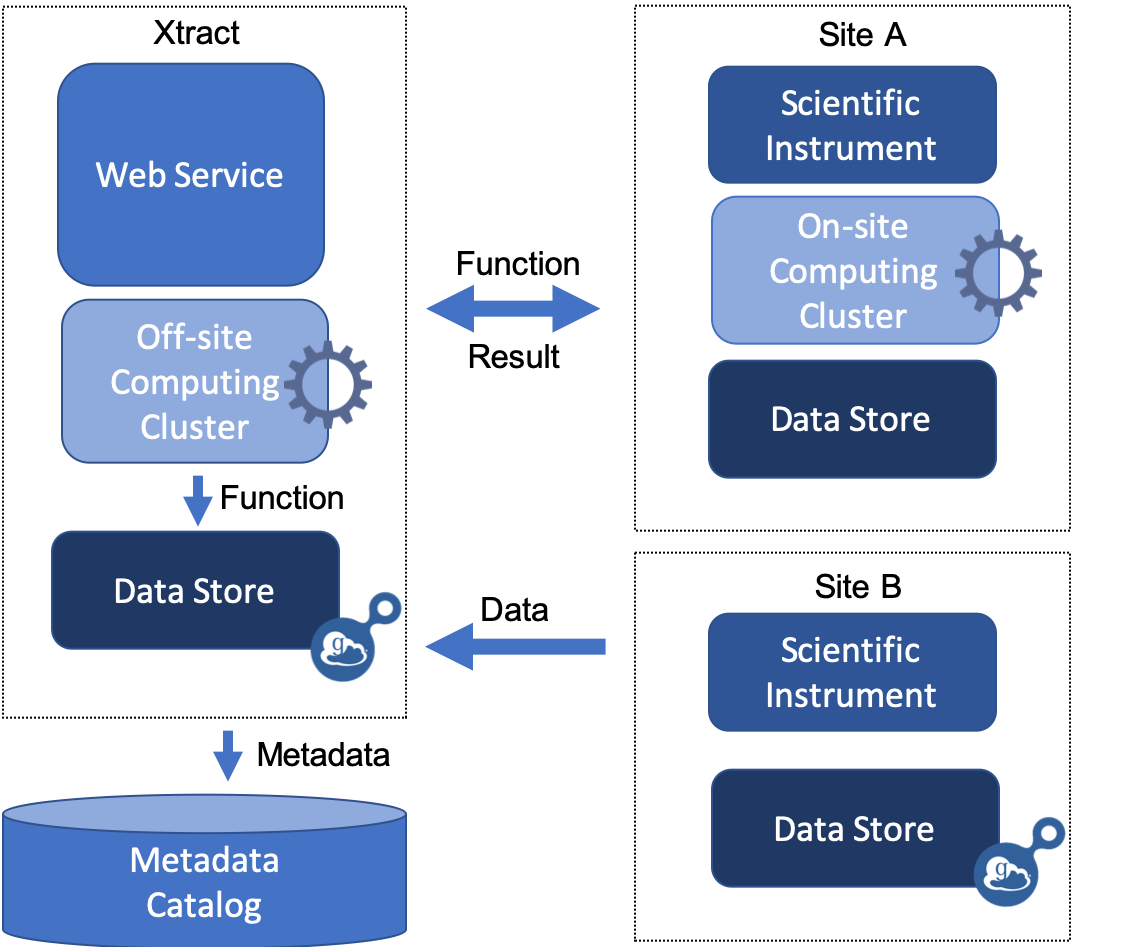
\includegraphics[scale=0.45]{figs/new-arch.png}
	\caption{Overview of the \name{} architecture. For \textit{Site A} functions are transmitted to the remote resource and performed on local computing resources, returning metadata to the \name{} service. \textit{Site B} lacks suitable local
	computing capabilities, requiring data to be staged to \name{} for analysis.}
	\label{fig:arch}
\end{figure}

\subsubsection{Metadata Extractors}
\name{} is designed to execute its extractors centrally or on edge storage systems near to where
data are stored. 
Our implementation uses the \funcx~\cite{chard2019serverless} FaaS platform 
to deploy and run extractors. 
\funcx{} is specifically designed to integrate with research computing 
cyberinfrastructure and enable a FaaS execution interface. 
\funcx{} builds upon the Parsl~\cite{babuji2019parsl} parallel programming library to 
manage the execution of functions in containers on arbitrary compute resources. 
\funcx{} enables \name{} to execute metadata extraction functions at any registered 
and accessible \funcx{} endpoint. 
We deploy the prototype with a co-located endpoint for central extraction
and use remotely deployed endpoints for edge extraction.

%The PetrelKube cluster is designed to enable analysis on data stored within Petrel. 
%PetrelKube 
%comprises 14 nodes, each with two E5-2670 CPUs, 128GB RAM, two 300GB hard drives in RAID 1, two 800GB Intel P3700 NVMe SSDs, 
%and 40GbE network interconnection. The \funcx{} endpoint is able to deploy and manage hundreds of \name{} extractor containers 
%to facilitate concurrent extraction.
%\name{} also integrates 
%both a  3.2PB object store accessible via Globus, called Petrel.
%%, and a Kubernetes cluster for elastically performing tasks, called PetrelKube. 
%%Petrel~\cite{petrel} is a. 
%Petrel provides six high-performance data transfer nodes 
%and is embedded in Argonne National Laboratory's 100+ Gbps network fabric. As metadata extraction requests are made to the 
%\name{} service, data is dynamically staged to Petrel for processing. 

%We deploy a \funcx{} endpoint to perform the metadata extraction tasks on the co-located Kubernetes cluster, 
%PetrelKube~\cite{petrelkube}. 

Each \name{} metadata extractor and its dependencies are wrapped in a Docker container
such that it can be executed in different locations. 
We have published each extractor container to \funcx{} and registered a \funcx{} function for 
each extractor. The function is responsible for invoking the extractor and returning the 
resulting metadata as a JSON dictionary. 

\funcx{} enables \name{} to reliably scale to thousands of nodes and deploy 
metadata extraction tasks on arbitrary computing resources. 
\name{} can make use of any accessible \funcx{} endpoint to process data at the edge, 
sending extractor codes and containers to the \funcx{} endpoint for execution. In addition, 
\funcx{} supports Singularity and Shifter, allowing \name{} extractors to be executed
on various high performance computing systems. 


\subsubsection{Data Staging}
%\kyle{Someone check this please. My read of the text here is that we have to download
%the data into the container in either edge or central mode? Can we also just mount 
%the local file system?} \ryan{On the edge it would just read from the file system.}

Irrespective of the extraction mode, either centralized or edge, the data
to be processed must be available to the deployed extractor container. 
In the case where data cannot be directly accessed within the container 
(e.g., where the container does not mount the local filesystem),
data are dynamically staged for processing. Each container includes
\name{} tooling to stage data in and out of the container. We use Globus as the 
basis for data staging, using Globus HTTPS requests, to securely download
remote data into the container. 

%\subsubsection{Usability}
%
%The \name{} service is designed to simplify data management for users and trivialize the task of cataloging and datasets. To 
%achieve this we provide a RESTful Web service and a Python SDK for programmatic access. User's send a request to the Web service 
%specifying a Globus-accessible dataset or directory. \name{} then initiates the transfer of data to Petrel and then manages the 
%application of the crawler and subsequent use of applicable metadata extractors. The resulting metadata is deposited into a Globus 
%Search~\cite{ananthakrishnan2018globus} index and is made available to the user.


\subsubsection{Security Model}

\name{} implements a comprehensive security model using Globus Auth~\cite{tuecke2016globus}. 
All interactions with the \name{} Web service are secured with Globus Auth. 
Users can authenticate with \name{} using one of 
several hundred identity providers, including many institutions. 
\name{} uses Globus Auth OAuth~2 flows to stage data on behalf
of authenticated users. \name{} first verifies a user identity, requests an access
token to perform data transfers on their behalf, and then uses Globus to stage
data from remote storage to the \name{} extractor. 
Finally, the resulting metadata are published into the search index using a Globus Search
access token. The search index is configured with a \textit{visible\_to} field, restricting
discovery to authenticated users.


\section{Evaluation}
\label{sec:eval}
We evaluate \name{} by extracting metadata from 
%extraction of metadata from MDF as the basis for 
%evaluating \name{}'s performance and usability. To this end, 
%we show that our 
%prototype extracts complete metadata of
more than \num{250000} files stored in MDF. 
% the 2.2 million files, and partial metadata for the rest. 
We deployed the \name{} service on AWS and deployed a private \funcx{} endpoint on ANL's
PetrelKube---a 14-node Kubernetes cluster. 
The MDF data are stored on the Petrel data service, a Globus-managed 3 PB data store at ANL. 
While Petrel and PetrelKube are located within the same network, they do
not share a file system. Thus, when executing extractors close to the data 
we still stage the data from Petrel to PetrelKube for processing.

In this section we first evaluate \name{}'s performance by crawling all files 
on the MDF as a means of initializing 
the downstream metadata extraction workflow and providing summary statistics about the data. 
We next profile the downstream
metadata extractor functions on hundreds of thousands of heterogeneous files in MDF.  
Finally, we illustrate the performance of batching
multiple files into one extractor function across multiple representative file types. 

% 5.1880962564547852267 hours to process
% 2215594 unique files
% Effective speed: 2215594 / (5.188096256454*3600)

\subsection{Crawling Performance}
First we crawl MDF to identify and record file locations, as well as general 
%physical 
attributes about 
each file such as size and extension.
\name{} manages the crawling process from the central \name{} service, employing a remote breadth-first search 
algorithm on the directory via Globus. % directory listings to inflate the search space.  
In processing MDF, \name{} crawled each of the 2.2 million files
in approximately \num{5.2} hours---at an effective rate of \num{119} files crawled per second. 
As part of crawling, \name{} generated descriptive treemaps about general attributes of the data. One such treemap 
illustrating the proportion of the most common extensions in MDF is shown in \figurename{~\ref{fig:treemaps}}. Here 
we observe that atomic structure (\emph{.xyz}), unknown (\emph{nan}), and image files (\emph{.tiff/.tif}) 
are most common in MDF relative to other types.

\begin{figure*}
	\includegraphics[scale=0.38]{figs/extension_treemap2.jpg}
	\caption{A treemap of the MDF extension frequency. The proportion of the size of each box relative to the entire
	treemap is equivalent to the proportion of the frequency of that file extension in MDF out of the 2.2 million total files}
    \label{fig:treemaps}
\end{figure*}


\subsection{File Type Training}
We next evaluate the time taken to perform the optional model training step for the file type extractor. 
Automated training of this model occurs by trying every extractor on each file 
in a 5-10\% subset of the total data set, denoting the first extractor that returned serviceable metadata without error. 
This extractor represents this file's label and the first 512 bytes the features for the random forests model. 
\name{} conducted such automated training on \num{110900} MDF files.
The entire label creation, feature collection, and training workflow took
approximately \num{5.3} hours.
We found that label generation constitutes a majority of this time, as
feature generation and model training total just 45 seconds. It is important to note that, in the future, increasing the 
number of PetrelKube pods concurrently serving feature label-collection functions can drastically
reduce the time taken to train the model.


\subsection{Extractor Performance}
We next evaluate the performance of \name{}'s extractors by invoking extraction functions on MDF's data.
We process a variety of file types including all available tabular and structured files and 
at least \num{25000} of each other type of file, selected randomly from MDF.
The performance of each extractor is summarized in \tablename{~\ref{tab:extractors}}.

\begin{table}[h]
	\caption{Extractor performance.} \label{tab:extractors}
\begin{center}
	\small
	\begin{tabular}{l c p{1.3cm} p{1.6cm} p{1.4cm}} 
 \hline
		\textbf{Extractor} & \# \textbf{Files} & \textbf{Avg. Size (MB)} & \textbf{Avg. Extract Time (ms)} & \textbf{Avg. Stage Time (ms)}\\ [0.5ex] 
 \hline
		\textbf{File Type} & 25,132         & 1.52 & 3.48 & 714 \\ 
 \hline
		\textbf{Images} & 76,925            & 4.17 & 19.30 & 1,198\\
 \hline
		 \textbf{Semi-strucured} & 29,850   & 0.38 & 8.97 & 412\\
 \hline
		\textbf{Keyword} & 25,997           & 0.06 & 0.20  & 346\\
 \hline
		\textbf{Materials} & 95,434         & 0.001 & 24 & 1,760\\
 \hline
		\textbf{Hierarchical*} & 3,855      & 695 & 1.90 & 9,150\\
 \hline
		\textbf{Tabular} & 1,227            & 1.03 & 113 & 625\\
 \hline
 
\end{tabular}
\end{center}
\end{table}

%\kyle{What do we want to say here?} \tyler{this?} \tyler{deleting cuz you're looking at it anyways ha}
We observe that a majority of extractor function invocations 
finish within milliseconds, and a majority of a file's round-trip 
processing time occurs due to file staging. This observation exemplifies
% crystallizes 
the need to
invoke functions near to data, directly mounted to file system 
housing the data, whenever possible.  Moreover we note that a few dozen large hierarchical files, 
exceeding 10 GB in size, were not processed due to ephemeral storage constraints on PetrelKube.
%Some large hierarchical files completed  (e.g., HDF and NetCDF files) that were not saved in a format that facilitates chunked reading require the 
%entire file to
%be loaded into memory when processed. As future work we will investigate the tradeoff between extracting metadata from 
%these files on resource-scarce nodes 
%versus transferring them to a location where they can be loaded entirely into memory. 

\begin{figure}
	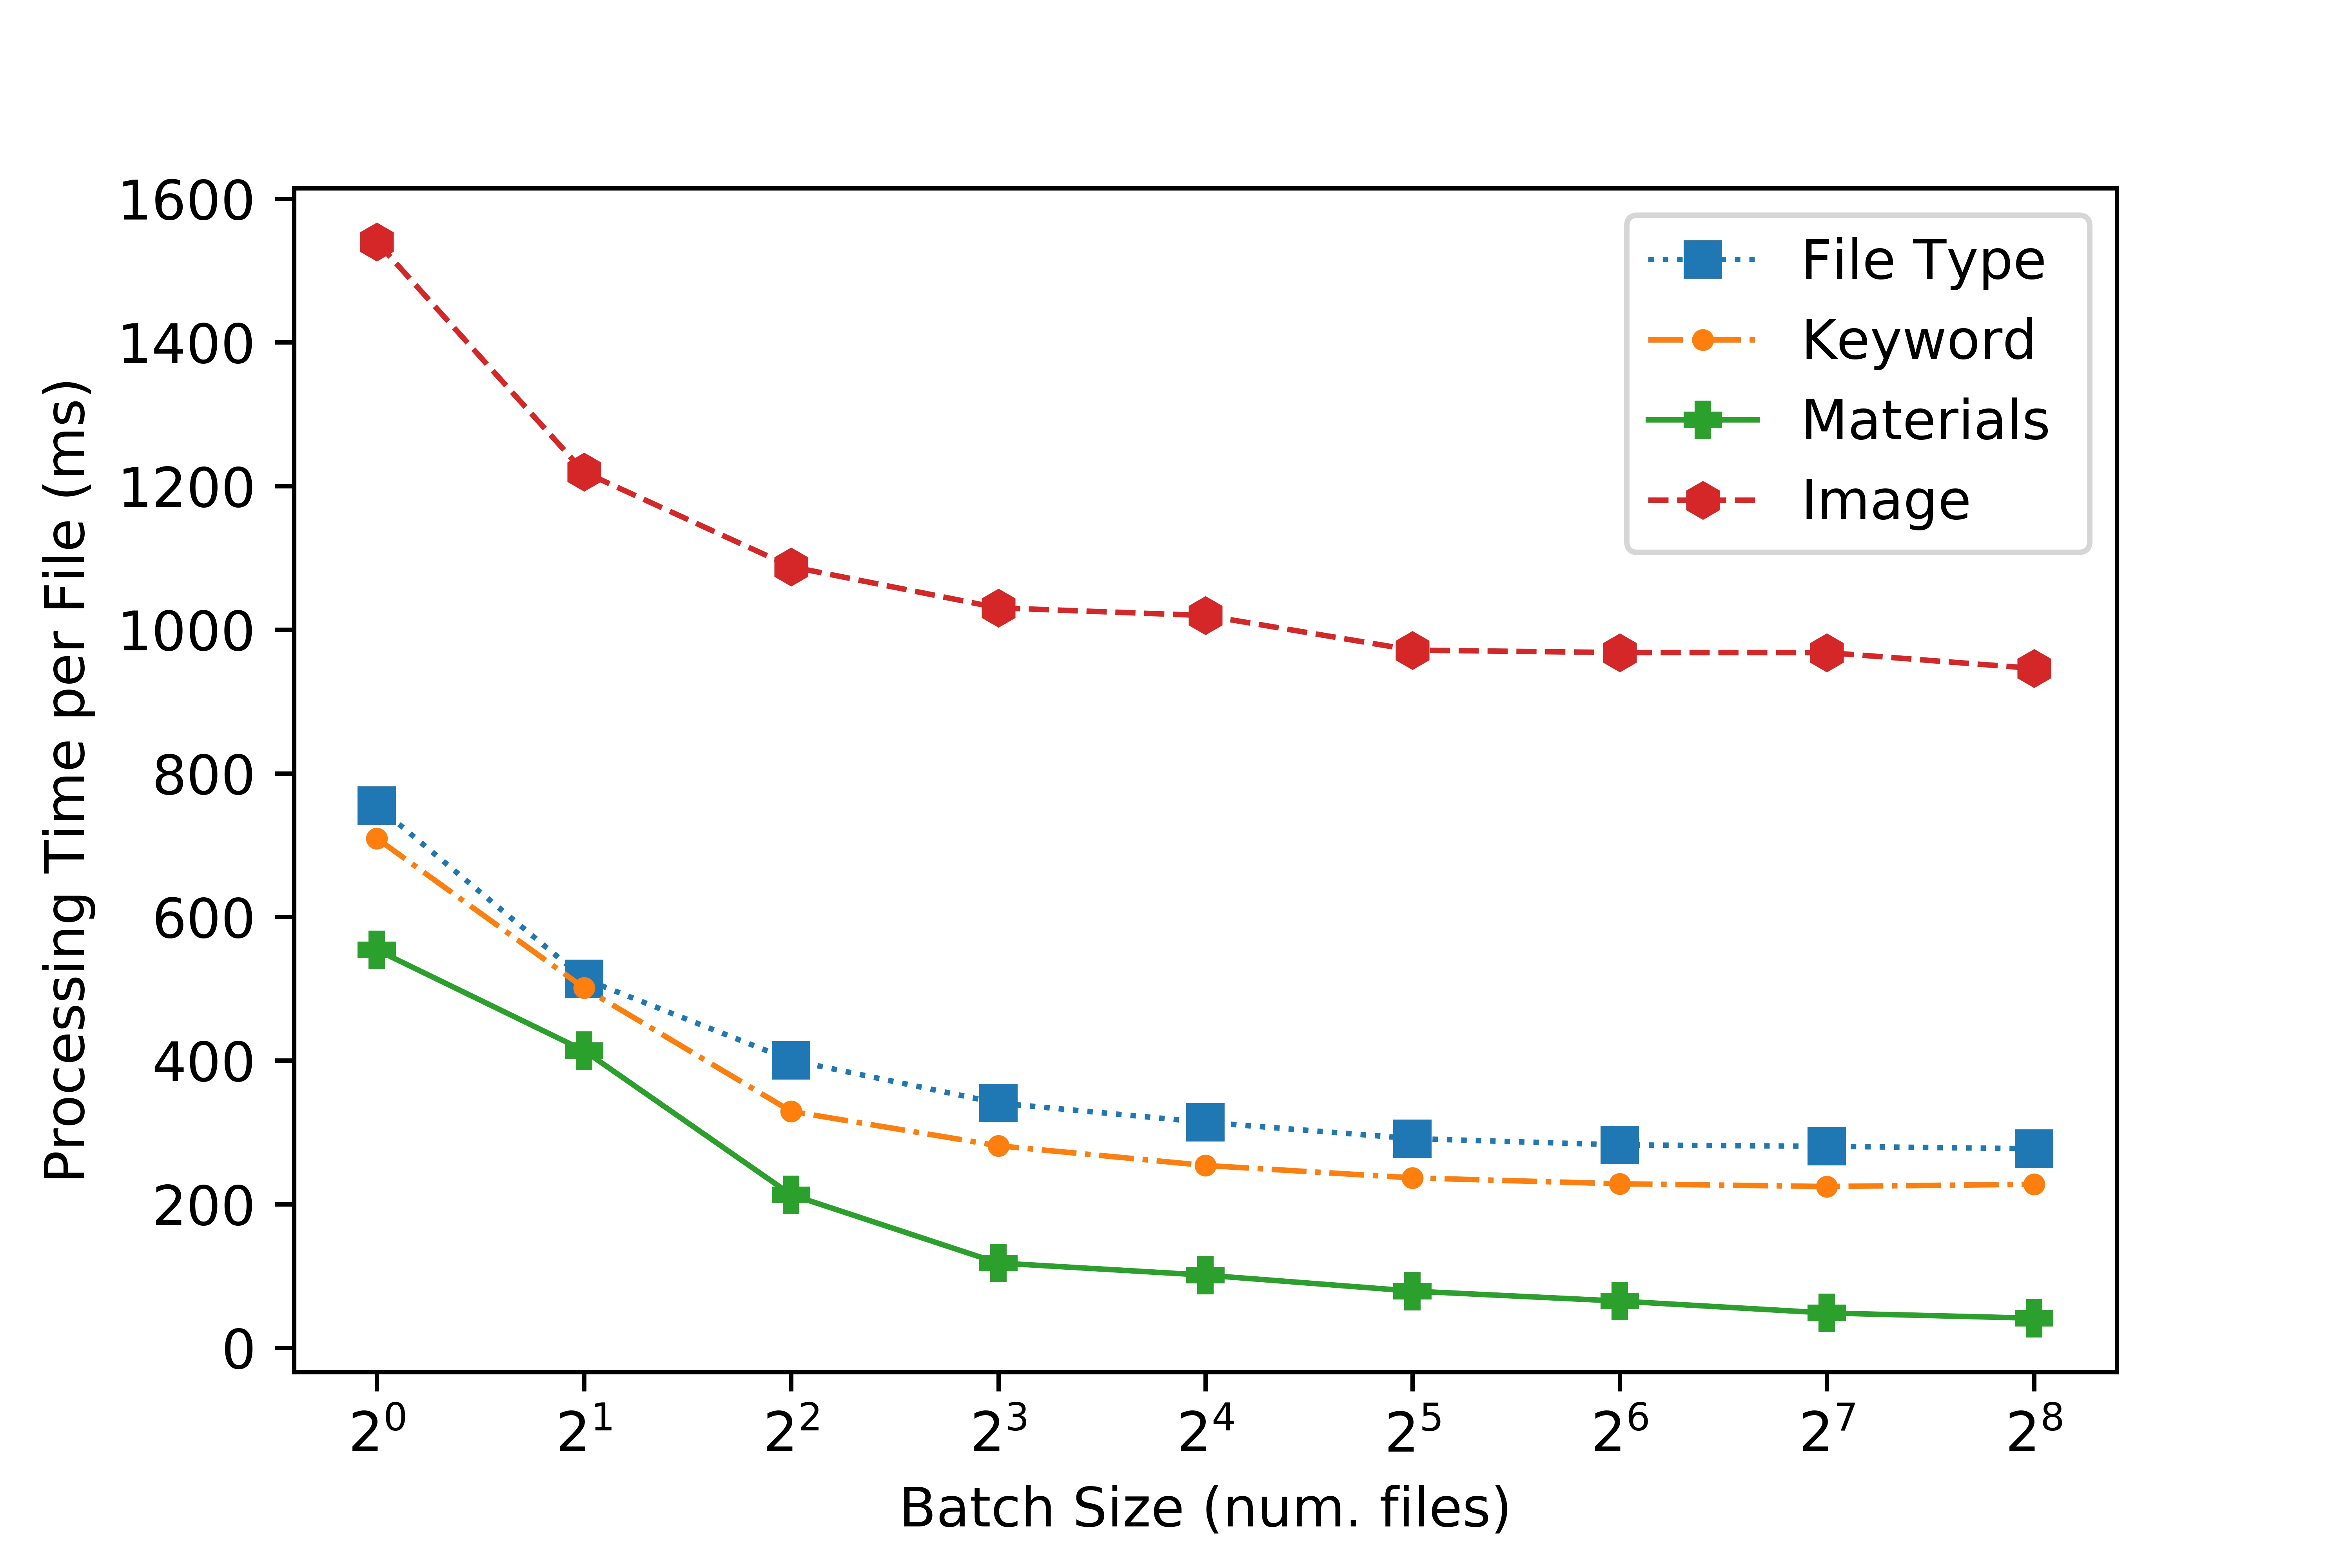
\includegraphics[scale=0.6]{figs/batch-times.jpg}
	\caption{Batching: extraction time per file (ms) on batches sized 1-256 for representative files processed by the 
	file type, image, keyword, and materials extractors}
    \label{fig:batching}
\end{figure}

Finally, we explore the benefits of batching multiple files 
into one function invocation request. We choose the four most applicable 
extractors: file type, keyword, images and materials. 
We randomly selected representative files of all four types, each within 2\% of the average
file sizes shown in Table~\ref{tab:extractors}. 
We implement batching by aggregating 1-256 files into a single \name{} request and
have modified the \funcx{} function to download and process files in parallel. 
Figure~\ref{fig:batching} shows that batching decreases the average time 
required to process a file as the batch size increases. 
Thus, batching can increase the performance of 
metadata extraction workflows, especially those requiring file transfers. 


\section{Related Work}
\label{sec:related}

\name{} builds upon a large body of work in both metadata extraction systems and serverless computing. 
\name{} is not the first to provide a scalable solution to extract metadata from datasets.
Pioneering research on data lakes developed methods for 
extracting standard metadata from nonstandard file types and formats~\cite{terrizzano2015data}. 
Most data lakes are designed with a specific target domain for which they are optimized, 
whether they primarily focus on transactional, scientific, or networked data. 
\name{} is designed to be easily extensible and therefore can be eaisly applied
to different domains. 
%for data without any standardization guarantees, 
%providing information on related, relevant data and their attributes.

We~\cite{wozniak15bigdata} and others~\cite{egan2003vizier, welter2013nhgri, irods, dataverse} have created 
systems to manage metadata catalogs that
support the organization and discovery of research data. However, these approaches typically 
require that users provide metadata and that curators continue to organize data over time. 
A number of systems exist for automatically extracting metadata from repositories. 
For example, ScienceSearch~\cite{rodrigo2018sciencesearch} uses 
machine learning techniques to extract metadata from a dataset served by the National Center for Electron Microscopy (NCEM). 
Most of data in this use case are micrograph images, but additional contextual metadata are derived from file system 
data and free text proposals and publications. Like \name{}, ScienceSearch 
provides a means for users to extensibly switch metadata extractors to suit a given dataset.  
Brown Dog~\cite{padhy2015brown} is an extensible metadata extraction platform, 
providing metadata extraction services for a number of 
disciplines ranging from materials science to social science.
Unlike \name{}, Brown Dog requires that files are uploaded for extraction. 
The Apache Tika toolkit~\cite{mattmann2011tika} is an open-source content and metadata extraction library. 
%While Tika does not yet exist as a service, it
Tika has a robust parser interface in which users can create and 
employ their own parsers in metadata extraction workflows. 
While Apache Tika has parsers that support thousands of file formats, the automated parser-to-file mapping 
utilizes MIME types to find suitable parsers for a file, which is often misleading for many scientific data
use cases. \name{} could be extended to support Tika extractors and to enable
execution on a serverless platform. %\ryan{Didn't you add tika as an xtract extractor? if so we should say it.}

While most related research performs metadata extraction to enable search,
\name{}-like systematic sweeps across repositories can also be used for analysis.  
For example, the Big Data Quality Control (BDQC) framework~\cite{deutsch2018bdqc} sweeps over 
large collections of biomedical data without regard to their meaning (domain-blind analysis) with the goal of
identifying anomalies.
BDQC employs a pipeline of extractors to derive properties of imaging, genomic, and clinical data.
While BDQC is implemented as a standalone system, the approach taken would be equally 
viable in \name{}.


\section{Conclusion}
\label{sec:conclusion}

%As scientific instruments and computing capabilities trend toward exascale, 
The growing volume, velocity, and variety of scientific data is becoming unmanageable.  
Without proper maintenance and management, data lakes quickly degrade 
into unorganized data swamps, lacking the necessary metadata for researchers 
to efficiently discover, use, and repurpose data. 
The growing size and heterogeneity of scientific data makes extracting rich 
metadata a complex and costly process, requiring a suite of customized extractors
and advanced extraction techniques. % often limited to those with access to HPC resources. 
We have described a serverless-based approach for metadata extraction, 
called \name{}. 
\name{} enables the scalable extraction of metadata from large-scale and distributed data lakes,
in turn increasing the value of data. 
We showed that our prototype can crawl and process hundreds of thousands of files from a multi-terabyte 
repository in hours, and that batching files and parallelizing file staging 
and extraction tasks can improve the performance of
%of round-trip 
metadata extraction times. 
%\tyler{@Kyle is the previous concrete enough? A little odd to slap a flat percentage on it given that the extractors are so different}

In future work we are focused on scaling the \name{} model and exploring the use
of \name{} on larger and globally distributed datasets. We will investigate strategies
for guiding extractor placement across scientific repositories, weighing 
data and extractor transfer costs to optimize placement. Finally, we
will extend \name{} to facilitate the integration of custom metadata extractors.
\begin{acks}

%This work was supported in part by Laboratory Directed Research and
%Development funding from Argonne National Laboratory under U.S. Department of
%Energy under Contract DE-AC02-06CH11357. 
This research used resources of the
Argonne Leadership Computing Facility, which is a DOE Office of Science User
Facility supported under Contract DE-AC02-06CH11357. 
We gratefully acknowledge the computing resources provided and 
operated by the Joint Laboratory for System Evaluation (JLSE) at Argonne National Laboratory. 

%\tyler{Ian, ny we are missing?}
%\kyle{Prob MDF} %and maybe RCC}

\end{acks}

%%
%% The next two lines define the bibliography style to be used, and
%% the bibliography file.
\bibliographystyle{ACM-Reference-Format}
\bibliography{wosc}


\end{document}
\endinput
%%
%% End of file `sample-authordraft.tex'.
